\uuid{amGb}
\exo7id{5201}
\titre{exo7 5201}
\auteur{rouget}
\organisation{exo7}
\datecreate{2010-06-30}
\isIndication{false}
\isCorrection{true}
\chapitre{Géométrie affine euclidienne}
\sousChapitre{Géométrie affine euclidienne du plan}
\module{Géométrie}
\niveau{L2}
\difficulte{}

\contenu{
\texte{
\label{exo:suprou7bis}
}
\begin{enumerate}
    \item \question{$h$ (resp. $h'$) est l'homothétie de centre $\Omega$ et de rapport $k$ (resp. $k'$) non nul. Déterminer la nature et les éléments caractéristiques de $h'\circ h$.}
    \item \question{$s$ (resp. $s'$) est la symétrie centrale de centre $\Omega$ (resp. $\Omega'$). Déterminer la nature et les éléments caractéristiques de $s'\circ s$.}
    \item \question{$s$ est la symétrie centrale de centre $\Omega$ et $t$ est la translation de vecteur $\overrightarrow{u}$. Déterminer la nature et les éléments caractéristiques de $t\circ s$.}
\reponse{
Soient $k$ et $k'$ deux réels non nuls, $\Omega$ et $\Omega'$ deux points (pas nécessairement distincts), puis $h$ (resp.$h'$) l'homothétie de centre $\Omega$ (resp. $\Omega'$) et de rapport $k$ (resp. $k'$).

Soient $M$ un point du plan, puis $M'=h(M)$ et $M''=h'(M')$.

\begin{align*}
M''&=\Omega'+k'\overrightarrow{\Omega'M'}=\Omega'+k'(\overrightarrow{\Omega'\Omega}+\overrightarrow{\Omega M'})
=\Omega'+k'\overrightarrow{\Omega'\Omega}+kk'\overrightarrow{\Omega M}\;(*)
\end{align*}

Chechons alors les points invariants par $h'\circ h$.

\begin{align*}
h'\circ h(M)=M&\Leftrightarrow\Omega'+k'\overrightarrow{\Omega'\Omega}+kk'\overrightarrow{\Omega M}=M
\Leftrightarrow-\overrightarrow{\Omega'M}+k'\overrightarrow{\Omega'\Omega}+kk'\overrightarrow{\Omega M}=\overrightarrow{0}\\
 &\Leftrightarrow(kk'-1)\overrightarrow{\Omega M}=(k'-1)\overrightarrow{\Omega\Omega'}\;(**)
\end{align*}

\begin{itemize}
[\textbf{1er cas.}] Si $kk'\neq1$, $(**)\Leftrightarrow\overrightarrow{\Omega M}=\frac{k'-1}{kk'-1}\overrightarrow{\Omega\Omega'}$, ce qui signifie que l'équation $(**)$ a une et eune seule solution que l'on note $\Omega''$, ou encore $h'\circ h$ a un et un seule point invariant, le point $\Omega''$ tel que 
$\Omega''=\Omega'+k'\overrightarrow{\Omega'\Omega}+kk'\overrightarrow{\Omega\Omega''}$.

Mais alors, l'égalié $(*)$ s'écrit pour tout point $M$

$$M''=\Omega'+k'\overrightarrow{\Omega'\Omega}+kk'\overrightarrow{\Omega M}
=\Omega'+k'\overrightarrow{\Omega'\Omega}+kk'\overrightarrow{\Omega\Omega''}+kk'\overrightarrow{\Omega''M}
=\Omega''+kk'\overrightarrow{\Omega''M}.$$

$h'\circ h$ est donc l'homothétie de rapport $kk'$ et de centre $\Omega''$. On doit noter que le centre $\Omega''$ est sur la droite $(\Omega\Omega')$.

\shadowbox{Si $kk'\neq1$,\;$h'\circ h$\; est une homothétie de rapport\;$kk'$.}
[\textbf{2ème cas.}] Si $kk'=1$, l'égalité $(*)$ s'écrit pour tout point $M$, $M''=\Omega'+k'\overrightarrow{\Omega'\Omega}+\overrightarrow{\Omega M}$ et donc

$$\overrightarrow{MM''}=\Omega'+k'(\Omega-\Omega')+(M-\Omega)-M=(1-k')\overrightarrow{\Omega\Omega'}.$$

Dans ce cas, $h'\circ h$ est la translation de vecteur $(1-k')\overrightarrow{\Omega\Omega'}$.
\end{itemize}

En résumé, \textbf{la comoposée de deux homothéties de rapport respectifs} $\bf{k}$ \textbf{et} $\bf{k'}$ \textbf{tous deux non nuls est une homothétie de rapport} $\bf{kk'}$ \textbf{si} $\bf{kk'}\neq1$ \textbf{et une tranlation si} $\bf{kk'=1}$ (ce résultat est à connaître).
C'est un cas particulier de la question précédente. Une symétrie centrale est une homothétie de rapport $-1$. Puisque $(-1)(-1)=1$, $s'\circ s$ est une translation. Son vecteur est $\overrightarrow{\Omega s'\circ s(\Omega)}=\overrightarrow{\Omega s'(\Omega)}=2\overrightarrow{\Omega \Omega'}$.

$$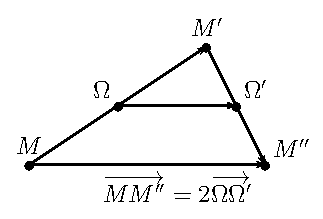
\includegraphics{../images/img005201-1}$$

\textbf{La composée de deux symétries centrales est une translation.}
Soit $\Omega'$ le point tel que $\overrightarrow{u}=2\overrightarrow{\Omega'\Omega}$, c'est-à-dire 
$\Omega'=\Omega-\frac{1}{2}\overrightarrow{u}$. Soit $s'$ la symétrie centrale de centre $\Omega'$. D'après 2), $s\circ s'$ est la translation de vecteur $2\overrightarrow{\Omega'\Omega}=\overrightarrow{u}$. Par suite, $s\circ t=s\circ s\circ s'=s'$.

\textbf{La composée d'une symétrie centrale et d'une translation est une symétrie centrale.}
}
\end{enumerate}
}
